\documentclass{jsarticle}
\usepackage{color}
\usepackage{bm}
\usepackage[height=26cm,width=16cm]{geometry} 
\usepackage{amsmath}
\usepackage{cases}
\usepackage[dvipdfmx]{graphicx}
\title{応数3}
\graphicspath{{./image/}}

\begin{document}

\section{12/21 問題4}
	ストークスの定理は関数の値が1/2ずつに別れて左右に速さvで進んでいく
	\begin{center}
		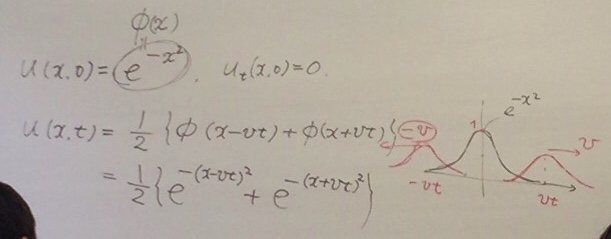
\includegraphics[width=7cm]{12_21_1.JPG}
	\end{center}
	最後のはcosを展開しただけ
	\begin{center}
		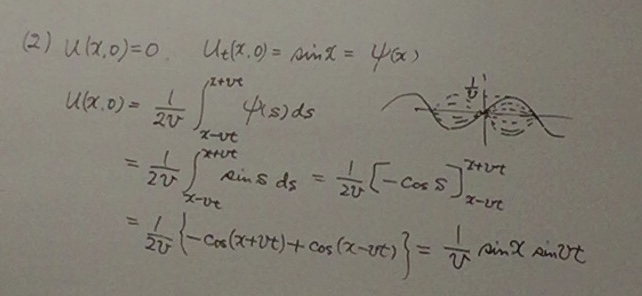
\includegraphics[width=7cm]{12_21_2.JPG}
	\end{center}
	上の式は無限空間、いまからのやつは有限の関数をかたっぽ有限でかたっぽゼロからの奇関数に広げるか、偶関数で広げるか
	\begin{center}
		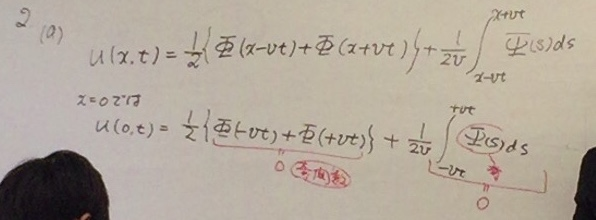
\includegraphics[width=7cm]{12_21_3.JPG}
	\end{center}
	$u_x(x,t)$は関数u(ここでは上の式)をxで偏微分
	\begin{center}
		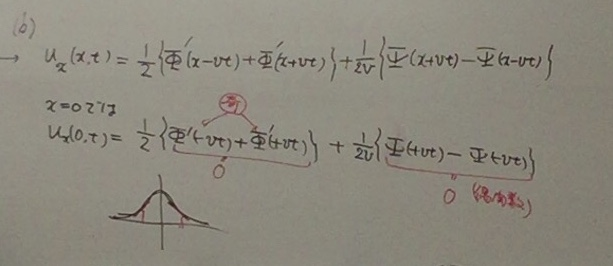
\includegraphics[width=7cm]{12_21_4.JPG}
	\end{center}
	φは偶関数だが、偶関数の微分は傾きだから奇関数となる\\
	
\end{document}